\section{Análisis de Circuito propuesto}

En esta sección se analiza el comportamiento de un circuito RLC serie a partir del material audiovisual de la clase. El objetivo es validar la teoría de resonancia mediante la observación de la respuesta en frecuencia y la comprobación analítica de los parámetros del sistema.

\subsection{Descripción del Circuito Prototipo}

El circuito analizado en el video consta de una fuente de tensión alterna senoidal conectada en serie con una resistencia, un inductor y un capacitor. Los valores nominales de los componentes son los siguientes:

\begin{itemize}
	\item \textbf{Voltaje de entrada ($V_{in}$):} $150\,V_{rms}$ a $0^{\circ}$.
	\item \textbf{Resistencia ($R$):} $15\,\Omega$.
	\item \textbf{Inductancia ($L$):} $10\,H$.
	\item \textbf{Capacitancia ($C$):} $10\,\mu F$.
\end{itemize}

% --- Espacio para captura del circuito ---
\begin{figure}[ht]
	\centering
	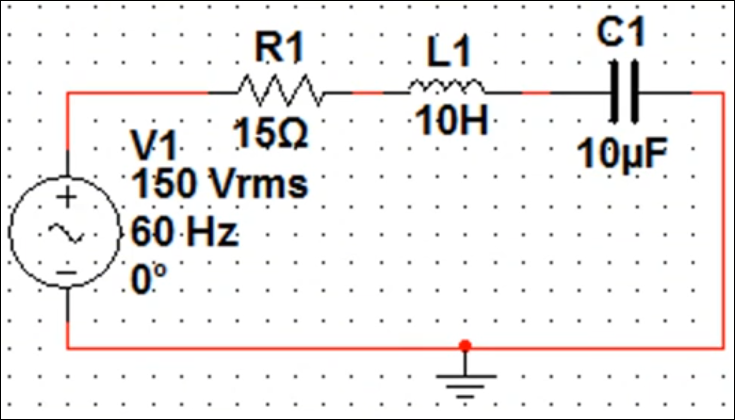
\includegraphics[width=0.7\textwidth]{assets/img/circuito_video.png}
	\caption{Configuración del circuito RLC serie analizado en el video.}
	\label{fig:circuito_video}
\end{figure}

\subsection{Comprobación Analítica de Resultados}

A continuación, se desarrolla el análisis matemático para verificar los resultados mostrados en la simulación del video.

\subsubsection{Frecuencia de Resonancia}
Para que el circuito entre en resonancia, la reactancia neta debe ser nula. Utilizando la expresión de la frecuencia angular de resonancia ($\omega_0$):

\begin{equation}
	\omega_0 = \frac{1}{\sqrt{LC}} = \frac{1}{\sqrt{(10\,H)(10 \times 10^{-6}\,F)}} = \frac{1}{\sqrt{10^{-4}}} = 100\,\text{rad/s}
\end{equation}

Convirtiendo a frecuencia en Hertz ($f_0$):

\begin{equation}
	f_0 = \frac{\omega_0}{2\pi} = \frac{100}{2\pi} \approx 15.915\,\text{Hz}
\end{equation}

Este resultado coincide con el valor de $15.92\,\text{Hz}$ presentado en el material audiovisual.

\subsubsection{Factor de Calidad (Q) y Ancho de Banda (BW)}
El factor de calidad define la selectividad del circuito:

\begin{equation}
	Q = \frac{\omega_0 L}{R} = \frac{(100\,\text{rad/s})(10\,H)}{15\,\Omega} = \frac{1000}{15} \approx 66.67
\end{equation}

El ancho de banda se determina como:

\begin{equation}
	BW = \frac{\omega_0}{Q} = \frac{100\,\text{rad/s}}{66.67} = 1.5\,\text{rad/s}
\end{equation}

\subsubsection{Frecuencias de Media Potencia ($\omega_1, \omega_2$)}
Dado que el factor de calidad es alto ($Q > 10$), las frecuencias de corte se pueden aproximar de manera simétrica respecto a $\omega_0$:

\begin{equation}
	\omega_1 = \omega_0 - \frac{BW}{2} = 100 - 0.75 = 99.25\,\text{rad/s}
\end{equation}
\begin{equation}
	\omega_2 = \omega_0 + \frac{BW}{2} = 100 + 0.75 = 100.75\,\text{rad/s}
\end{equation}

\subsubsection{Análisis de Potencia en Frecuencias Críticas}
En resonancia, la impedancia es mínima e igual a $R$ ($15\,\Omega$), por lo que la corriente es máxima: $I_{max} = 150\,V / 15\,\Omega = 10\,A$.

\begin{itemize}
	\item \textbf{Potencia en $\omega_0$ ($P_0$):} 
	\begin{equation} P_0 = I_{max}^2 \cdot R = (10\,A)^2 \cdot 15\,\Omega = 1500\,W \end{equation}
	\item \textbf{Potencia en $\omega_1$ y $\omega_2$ ($P_{1,2}$):} Por definición, en estas frecuencias la potencia se reduce a la mitad:
	\begin{equation} P_1 = P_2 = \frac{P_0}{2} = 750\,W \end{equation}
\end{itemize}

% --- Espacio para la gráfica de Bode ---
\begin{figure}[ht]
	\centering
	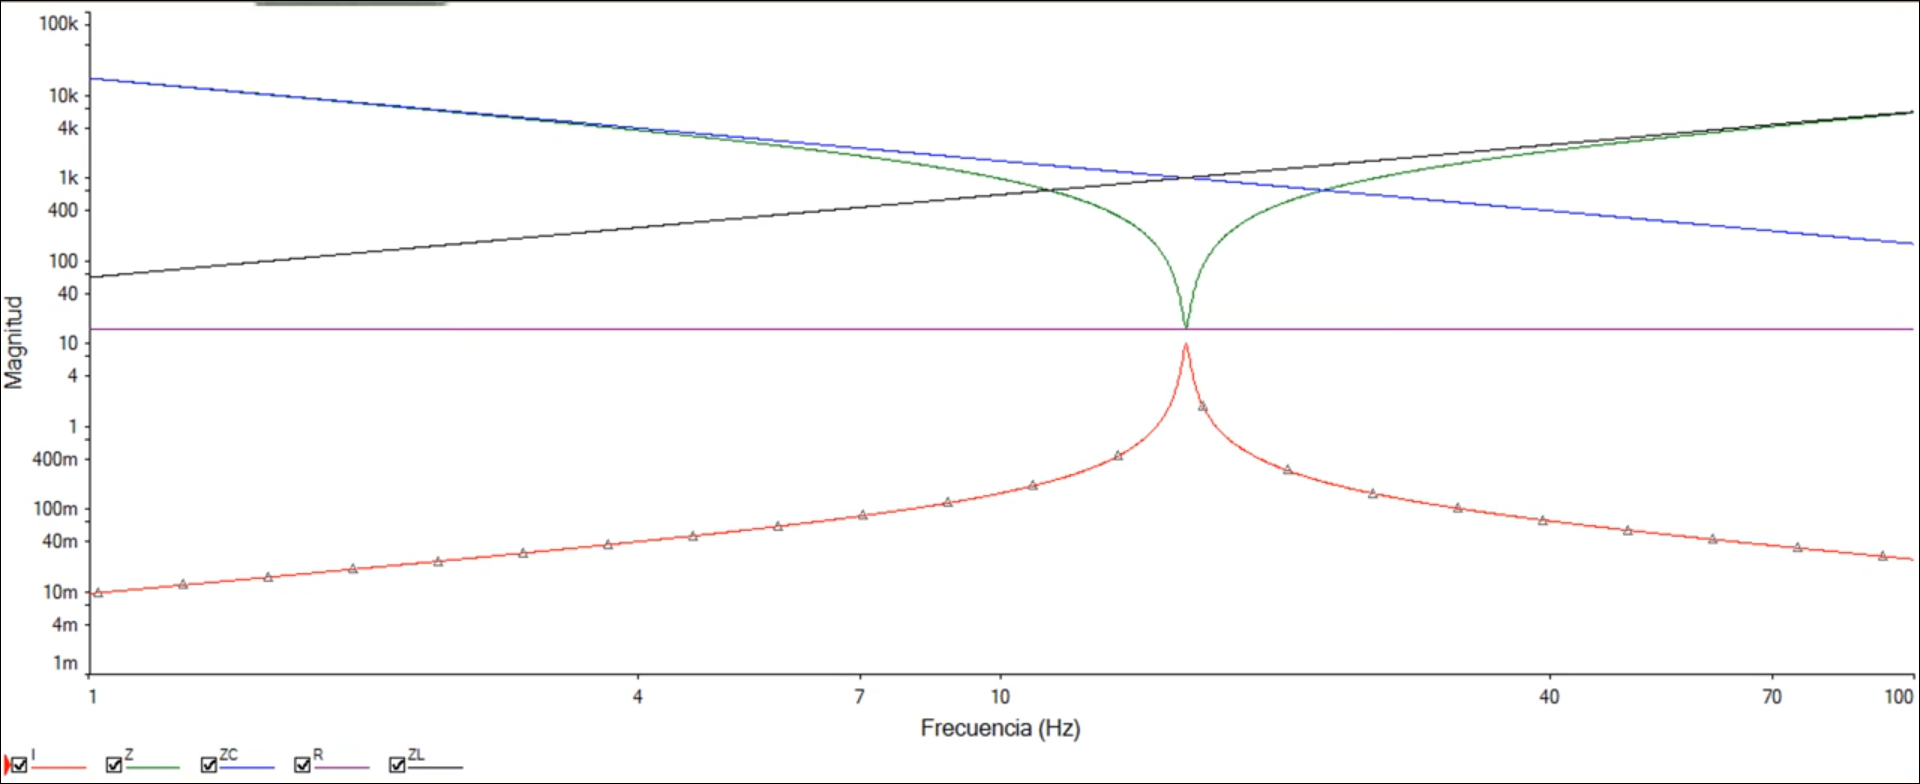
\includegraphics[width=0.8\textwidth]{assets/img/diagrama_bode_video.png}
	\caption{Curvas de magnitud de impedancia y corriente obtenidas en el video.}
	\label{fig:bode_video}
\end{figure}

\subsection{Explicación de Resultados}

Como se observa en la Figura \ref{fig:bode_video}, la curva de corriente (en rojo) presenta un pico pronunciado exactamente en la frecuencia de resonancia calculada ($15.92\,\text{Hz}$), donde alcanza un valor de $10\,A$. Simultáneamente, la curva de impedancia total (en verde) alcanza su punto mínimo, igualándose a la resistencia del circuito ($15\,\Omega$).

El alto valor del factor de calidad ($Q \approx 66.67$) explica por qué el pico de resonancia es tan agudo y el ancho de banda es tan estrecho ($1.5\,\text{rad/s}$). Esto indica una alta selectividad del circuito, donde la potencia se concentra fuertemente en una banda de frecuencias muy pequeña alrededor de $\omega_0$. Los resultados matemáticos validan con precisión la evidencia visual del video, demostrando que en las frecuencias de corte $\omega_1$ y $\omega_2$, el sistema efectivamente opera a media potencia debido a la reducción de la corriente por un factor de $1/\sqrt{2}$.